\documentclass{article}
\usepackage[utf8]{inputenc}
\usepackage[T1]{fontenc}
\usepackage{graphicx}
\graphicspath{ {./images/} }

\usepackage{tocloft}

\setlength{\parskip}{1em}
\renewcommand{\contentsname}{Spis treści}
\newcommand{\myparagraph}[1]{\paragraph{#1}\mbox{}\\\\}


\title{Zadanie projektowe nr 1 \\ Badanie efektywności operacji dodawania, usuwania oraz wyszukiwania elementów w różnych strukturach danych.}

\author{Leszek Błażewski, 241264}
\date{Tydzień nieparzysty 9:15}

\begin{document}

\maketitle
\thispagestyle{empty}

\newpage{}
\setcounter{page}{1}


\tableofcontents

\newpage{}

\section{Wstęp teoretyczny}

Celem przeprowadzonego eksperymentu było zbadanie efektywności podstawowych operacji takich jak wstawianie, wyszukiwanie oraz usuwanie elementu w postaci liczby cztero bajtowej do wybranej struktury danych.\linebreak
Wszystkie ze struktur zostały zaimplementowane przy użyciu szablonów, jako osobne obiekty w języku C++, dzięki czemu mogą zostać wykorzystane do przechowywania kluczy reprezentujących różne typy danych.

Badaną wielkością było asymptotyczne tempo wzrostu konkretnych operacji, zapisywane za pomocą notacji dużego $\mathcal{O}$, w celu późniejszego opisu złożoności obliczeniowej danych operacji.


\subsection{Tablica z realokacją pamięci}

Tablica jest strukturą danych zawierająca klucze, z których każdy jest \linebreak identyfikowalny przez konkretny indeks tablicy. Dostęp do kolejnych elementów tablicy odbywa się poprzez odwoływanie się do danego indeksu na podstawie, którego wyłuskiwany jest element.
W przeprowadzonych badaniach \linebreak zaimplementowana została tablica z realokacją pamięci przy usuwaniu oraz wstawianiu klucza w celu zaoszczędzenia pamięci.

\subsubsection{Wstawianie elementu} 

\myparagraph{Początek tablicy}
W celu wstawienia nowego klucza na początek tablicy tworzona jest nowa tablica o rozmiarze o 1 większym w której wszystkie klucze przesunięte zostają o jeden indeks do przodu a nowy klucz zajmuje miejsce o indeksie 0. Złożoność obliczeniowa takiej operacji zależy od wielkości tablicy, ponieważ wszystkie dane muszą zostać jednakowo przesunięte o jedną pozycję, przez co złożoność operacji wynosi $\mathcal{O}(n)$.
 
\myparagraph{Środek tablicy} 
Operacja wstawiania elementu pomiędzy inne elementy tablicy polega na alokacji nowej tablicy, przekopiowaniu wszystkich elementów do danego indeksu. Następnie wstawienie zadanego elementu na podany indeks. Ostatecznie przekopiować należy wszystkie pozostałe elementy od zadanego indeksu do końca ówczesnej tablicy. Złożoność obliczeniowa podanej operacji również jest liniowa, w związku z czym notacja dużego $\mathcal{O}$ wynosi $\mathcal{O}(n)$.

\myparagraph{Koniec tablicy} 
W tym przypadku nie ma potrzeby przesuwania elementów tablicy, co skutkuje zmniejszenie czasu wykonywania operacji, jednak nadal niezbędna jest realokacja pamięci. 
Złożoność obliczeniowa w tym przypadku również pozostaje bez zmian w związku z niezmienną potrzebą realokacji całej tablicy, w celu wstawienie \linebreak elementu na ostatnim indeksie. Złożoność operacji wynosi $\mathcal{O}(n)$.
 
\subsubsection{Usuwanie elementu}

\myparagraph{Początek tablicy}
Usuwanie jest operacją podobną do wstawiania, z tą różnicą, że przy usuwaniu z początku tablicy, realokujemy pamięć o mniejszym rozmiarze o 1 i przesuwamy wszystkie klucze o jeden indeks w dół z pominięciem indeksu 0. 
Ze względu na realokację i przesunięcie wszystkich elementów złożoność operacji również wynosi $\mathcal{O}(n)$.
 
\myparagraph{Środek tablicy} 
Operacja jest przeprowadzana w sposób analogiczny do dodawania elementu pomiędzy inne elementy w tablicy.
Alokowana jest nowa tablica o wielkości o jeden mniejszej do której przepisywane są wartości do danego indeksu. Następnie wartości znajdująca się na zadanym indeksie jest omijana, a pozostałe elementy kopiowane są do nowo zaalokowanej tablicy. Złożoność operacji wynosi $\mathcal{O}(n)$.


\myparagraph{Koniec tablicy} 
W tym przypadku również różnica jak przy wstawianiu. Czas wykonania krótszy ponieważ nie trzeba przesuwać wartości, jednak czas realokacji pozostaje bez zmian. Złożoność pozostaje bez zmian i wynosi $\mathcal{O}(n)$.
 
\subsubsection{Wyszukiwanie zadanego elementu} 

Każdy kolejny klucz w tablicy porównywany jest z szukanym kluczem do momentu znalezienia szukanej wartości, czyli w najgorszym wypadku trzeba przeszukać całą tablicę gdy wartość szukanego klucza nie znajduje się w tablicy, lub znajduje się na ostatniej pozycji.
Złożoność obliczeniowa w tym przypadku wynosi $\mathcal{O}(n)$. Wraz ze wzrostem liczby elementów czas poszukiwań rośnie liniowo.


\subsection{Lista dwukierunkowa}
 
Lista dwukierunkowa jest strukturą danych składającą się z sekwencyjnie połączonych ze sobą elementów. Każdy z elementów zawiera przechowywany klucz oraz dwa pola wskazujące na element poprzedni oraz następny na liście.\linebreak Przechowywanie wskaźnika na element następny oraz poprzedni pozwala na poruszanie się zarówno w przód jak i w tył po liście. Klasa reprezentująca listę przechowuje wskaźnik wskazujący na pierwszy element - head oraz wskaźnik identyfikujący ostatni element - tail, których odpowiednio poprzednikiem oraz następnikiem są wskaźniki na wartość pustą. W przypadku języka C++ w wersji 11 jest to nullptr.

\subsubsection{Wstawianie elementu} 
 
\myparagraph{Początek listy}
W przypadku wstawiania na początek listy, nowy element staje się głową a ówczesny pierwszy element zostaje elementem kolejnym. Operacja ta nie jest czasochłonna, ponieważ wystarczy odpowiednio podmienić wskaźniki w taki sposób aby nowy element wskazywał na ówczesną głowę, natomiast ówczesna głowa jako element poprzedni wskazuje na nowy element. Złożoność czasowa takiej operacji jest stała, niezależna od ilości elementów, zawsze musimy wykonać jedynie operacje opisane powyżej. Złożoność operacji wynosi $\mathcal{O}(1)$.

\myparagraph{Środek listy} 
W przypadku kiedy chcemy wstawić nowy element w środek listy, musimy najpierw odnaleźć element który obecnie się tam znajduje, co jest tym bardziej czasochłonne im więcej elementów znajduję się w liście, ponieważ musimy przejść przez każdy poprzedni element, ze względu na fakt, że nie dysponujemy bezpośrednim indeksem za który należy wstawić nowy element. Następnie tworzymy nowe połączenia między nowym elementem, a jego następnikiem i poprzednikiem. 
Złożoność w tym wypadku nie jest już stała, jak miało to miejsce przy wstawianiu na początek listy, lecz jest liniowa, ze względu na iterację doprowadzającą, do żądanego miejsca na liście. Złożoność operacji wynosi $\mathcal{O}(n)$.

\newpage

\myparagraph{Koniec listy} 
Z przyjętych założeń implementacji listy jako obiektu przetrzymującego wskaźnik na pierwszy oraz ostatni element wnioskować możemy że czas wstawiania\linebreak elementu na koniec listy jest analogiczny do czasu dodawania elementu na pierwszej pozycji. Operację jaką należy wykonać to ustawienie wskaźnika na następny element obecnego ogona na nowy element, natomiast nowo dodany element wskazywać musi na ówczesny ogon. Złożoność operacji nie zależy od liczby przechowywanych elementów w liście, dlatego wynosi $\mathcal{O}(1)$.

\subsubsection{Usuwanie elementu}
 
\myparagraph{Początek listy} 
Przy usuwaniu z początku listy, jedyne operacje jakie musimy wykonać to przemianowanie drugiego elementu listy na element pierwszy, poprzez ustawienie jego pola wskaźnika na poprzednika na adres pusty, oraz dealokację poprzedniego pierwszego elementu. 
Operacja ta ma złożoność obliczeniową stałą, liczba elementów listy nie wpływa na szybkość jej wykonywania, w związku z czym wynosi $\mathcal{O}(1)$.
 
\myparagraph{Środek listy}
Tak samo jak w przypadku wstawiania elementu w środek listy tutaj również musimy odnaleźć element środkowy listy, co wraz z wzrostem elementów staje się coraz to bardziej czasochłonne. Po odnalezieniu elementu o dany kluczu, tworzymy nowe wiązania między jego następnikiem i poprzednikiem, a następnie element ten dealokujemy. Złożoność obliczeniowa wzrasta wraz ze wzrostem liczby elementów ze względu na potrzebę iteracji przez kolejne elementy listy. Złożoność operacji wynosi $\mathcal{O}(n)$.
 
\myparagraph{Koniec listy} 
Operacja jest analogiczna do wstawiania elementu na ostatnią pozycję.\linebreak Dzięki wskaźnikowi na ostatni element (tail), wystarczy ustawić wskaźnik jego poprzednika na element pusty a następnie zdealokować ogon. Operacja ta jest niezależna od liczby elementów na liście, w związku z czym wynosi $\mathcal{O}(1)$.
 
\subsubsection{Wyszukiwanie zadanego elementu} 
 
\myparagraph{Przeszukiwanie całej listy} 
Każdy kolejny klucz przechowywany przez elementy w liście porównywany jest z szukanym kluczem do momentu znalezienia szukanej wartości, czyli w najgorszym wypadku gdy klucz znajduje się na końcu listy lub nie występuje na liście, przeszukać należy całą listę. Operację tą można przyśpieszyć jeśli wiemy w której części listy leży zadany element, ponieważ iterować możemy zarówno od końca jak i od początku struktury.
W ogólnym przypadku złożoność obliczeniowa operacji jest liniowa i wynosi $\mathcal{O}(n)$.

\subsection{Kopiec maksymalny}

Kopiec jest strukturą danych przybierającą formę drzewa binarnego prawie pełnego. W zależności od rodzaju kopca, minimalny lub maksymalny, gdzie odpowiednio każdy syn jest większy lub mniejszy od swojego rodzica. W skutek tego otrzymujemy kopiec maksymalny lub minimalny gdzie odpowiednio w korzeniu przechowywana jest wartość największa lub najmniejsza. Wysokość kopca obliczana jest na podstawie wzoru: $\log_{2}(n)$, gdzie $n$ to ilość przechowywanych kluczy. Podczas implementacji kopiec reprezentowany jest jako tablica, której kolejne elementy zachowują odpowiednią relację, spełniającą warunek kopca. Przedstawione poniżej operacje opisane zostały dla kopca maksymalnego, lecz operacje te mają swoje analogiczne odzwierciedlenie dla kopca minimalnego.


\subsubsection{Wstawianie elementu} 
 
W przypadku kopca operacja wstawiania nie jest rozdzielana na konkretne pozycje, wartość wstawiana jest zawsze na miejsce za ostatnim elementem kopca, a następnie krok po kroku nowa wartość jest przesuwana w górę drzewa, poprzez porównanie nowego elementu z jego rodzicem i ich zamianie miejscami, jeżeli własności kopca nie są zachowane. W najgorszym przypadku, gdy nowa wartość jest największa w kopcu złożoność obliczeniowa operacji wstawiania to $\mathcal{O}(log(n))$, ponieważ tyle właśnie operacji zamiany elementów trzeba wykonać.

\subsubsection{Usuwanie elementu} 

W przypadku usuwania nie wyróżnia się usuwania z konkretnych pozycji, lecz jedynie usuwanie elementu największego znajdującego się w korzeniu. W celu usunięcia korzenia, zamienia się wartościami klucz korzenia z elementem ostatnim w drzewie a następnie usuwa się ostatni element. Później przeprowadzany jest ciąg operacji mający na celu przywrócenie własności kopca, poprzez \linebreak odpowiednie przesuwanie elementu w dół drzewa.
Operacja ta ma złożoność czasową logarytmiczną $\mathcal{O}(log(n))$), ponieważ po zamianie korzenia z elementem ostatnim, zazwyczaj trzeba przesunąć nową wartość korzenia na sam dół drzewa, czyli wykonać $log_2(n)$ operacji zamiany.

Ze względu na wymogi zadania, usuwanie elementu odbywa się poprzez wyszukanie elementu o zadanym kluczu. Następnie dany element zamieniany jest z ostatnim elementem w kopcu. Później dochodzi do operacji naprawy kopca odpowiednio w dół lub w górę w zależności od usuniętego elementu. 
 
\subsubsection{Wyszukiwanie zadanego elementu} 

Każdy kolejny klucz przechowywany w kopcu porównywany jest z szukanym kluczem do momentu znalezienia szukanej wartości, czyli w najgorszym wypadku trzeba przeszukać cały kopiec gdy wartość klucza szukanego nie znajduje się w kopcu lub znajduje się na ostatniej pozycji w tablicy reprezentującej kopiec.
Złożoność operacji wynosi $\mathcal{O}(n)$.
 
\subsection{Drzewo BST}

Drzewo przeszukiwań binarnych jest strukturą drzewiastą, w której dla każdego węzła x zachodzi poniższy warunek:
wartość każdego elementu leżącego w lewym poddrzewie węzła x jest nie większa niż wartość węzła x, natomiast wartość każdego elementu leżącego w prawym poddrzewie węzła x jest nie mniejsza niż wartość tego węzła. Wartym odnotowania jest fakt iż drzewo BST w przeciwieństwie do kopca nie jest drzewem pełnym, w związku z czym liczba poziomów niezrównoważonego drzewa może przekroczyć wartość $log_2(n)$.

W programie struktura ta implementowana jest jako ciąg wskaźników struktur z których każda zawiera trzy elementy:
wskaźnik na rodzica, lewego oraz prawego syna i klucz który przechowuje daną wartość. Dostęp do drzewa odbywa się poprzez wskaźnik na jego korzeń.

\subsubsection{Wstawianie elementu}

Proces wstawiania elementu dzieli się na dwa zasadnicze podpunkty: pierwszy z nich to proces wyszukiwania miejsca dla nowego elementu poprzez porównywanie kolejnych kluczy w drzewie, gdzie ze względu na wynik porównania przesuwamy się odpowiednio w dół drzewa. Następnie wystarczy poprawnie ustawić wskaźniki w nowym elemencie oraz jego rodzicu. Gdy drzewo jest zrównoważone operacja dodawania elementu ma złożoność równą  $\mathcal{O}(log(n))$. W najgorszym przypadku złożoność operacji wynosi $\mathcal{O}(n)$.

\subsubsection{Usuwanie elementu}

W pierwszej kolejności wyszukać należy węzeł o zadanym kluczu a następnie należy usunąć go z struktury.
Algorytm usuwania elementu o zadanym kluczu z drzewa BST dzieli się na trzy zasadnicze przypadki:

\begin{itemize}
    \item Usuwany węzeł jest liściem.
    \item Usuwany węzeł posiada tylko jednego syna.
    \item Usuwany węzeł posiada dwóch synów.
\end{itemize}

W pierwszym przypadku wystarczy odłączyć węzeł od drzewa i zdealokować pamięć którą zajmuje.
W drugim przypadku wystarczy zastąpić usuwany węzeł jego synem, po czym węzeł usuwamy z pamięci.
Ostatni przypadek wymaga znalezienia następnika usuwanego węzła w drzewie. Następnik to wartość, która jest najmniejszą wartością z pozostałych w drzewie ale jest większa bądź równa usuwanemu elementowi.Po znalezieniu następnika przenosimy dane z jego węzła do usuwanego węzła po czym usuwamy następnik

Wyszukiwanie następnika podzielić można na dwa przypadki:
\begin{enumerate}
    \item Węzeł posiada prawego syna.
    \item Węzeł nie posiada prawego syna.
\end{enumerate}

Jeśli dany węzeł posiada prawego syna to jego następnikiem jest węzeł o minimalnym kluczu w poddrzewie, którego korzeniem jest prawy syn danego węzła. Jeżeli węzeł nie posiada prawego syna to poruszamy się w górę drzewa tak długo aż znajdziemy pierwszego ojca, dla którego nasz węzeł leży w lewym poddrzewie. Natomiast jeśli węzeł nie posiada prawego syna a idąc w górę dochodzimy do korzenia a następnie do adresu $NULL$, na które wskazuje pole parent korzenia, to dany węzeł posiada klucz o największej wartości i nie posiada on następnika. Złożoność operacji wynosi $\mathcal{O}(n)$.

\subsubsection{Wyszukiwanie zadanego elementu}

Główną zaletą drzewa BST jest liniowy czas przeszukiwań, ponieważ poprzez porównywanie wyszukiwanego elementu z obecnym kluczem w drzewie schodzimy tylko jedną ścieżką w dół struktury. Dobrze zbudowane drzewo binarne posiada złożoność obliczeniową wyszukiwania równą $\mathcal{O}(log(n))$. W najgorszym przypadku gdy drzewo nie jest zrównoważone złożoność operacji wynosi $\mathcal{O}(n)$.

\subsubsection{Algorytm DSW}

W przypadku dodawanie elementów na przykład o wyłącznie rosnących kluczach, drzewo przybrać może postać listy liniowej, tracąc w ten sposób wszystkie swoje zależności. Algorytm równoważenia drzewa polega na zminimalizowaniu liczby poziomów drzewa poprzez odpowiednie rotacje na węzłach. Algorytm DSW polega na początkowej rotacji węzłów w taki sposób aby z drzewa utworzyć listę liniową a następnie na co drugim węźle dokonywana jest rotacja elementów w lewo, która gwarantuje utworzenia drzewa o minimalnej licznie poziomów, co zapewnia złożoność operacji przeszukiwania równą $\mathcal{O}(log(n))$. Złożoność algorytmu DSW wynosi $\mathcal{O}(n)$.


\section{Plan eksperymentu}

\begin{itemize}
    \item Językiem programowania użytym w eksperymencie był $C++$ w standardzie ISO $C++11$.
    \item Badanie poszczególnych operacji zostało przeprowadzone na losowo generowanych zestawach danych zawierających klucze z przedziałów: \\$[10,100],[1,INTMAX], [INTMIN+100,INTMAX-100]$
    \item Losowe liczby z podanych przedziałów generowane były przy użyciu biblioteki random.
    \item Dla wszystkich struktur oprócz drzewa BST badania zostały przeprowadzone dla kolejnych wielkości struktur: $100000, 350000, 600000 ... 2100000$, natomiast dla drzewa ze względu na dłuższy czas wykonywania operacji przyjęto wielkości równe $1000,3500,6000 ... 21000$.
    \item Ilość powtórzeń wykonania każdej operacji wynosił $100$.
    \item Otrzymanym wynikiem jest zmierzony czas podzielony przez ilość wykonanych operacji wyrażony w nanosekundach.
    \item Czas wykonania operacji mierzony był przy użyciu biblioteki chrono za pomocą funkcji $std::chrono::high\_resolution\_clock$.
    \item Zgodnie z zaleceniami prowadzącego operacja dodawania i usuwania elementów z kopca nie realokowała tablicy przechowującej kopiec.
    \item Operacje dodawania oraz usuwania elementów do drzewa BST zostały zmierzone wraz z algorytmem DSW w celu zachowania właściwości drzewa dla podanych operacji.
\end{itemize}

\section{Wyniki}

Wszystkie obliczone czasy przedstawione zostały w nanosekundach.

\subsection{Tablica}

\subsubsection*{Wstawianie elementu na początek}
\begin{figure}[h!]

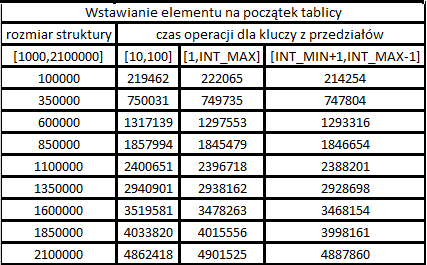
\includegraphics{images/TAB_POCZATEK.png}

\end{figure}

\begin{figure}[h!]
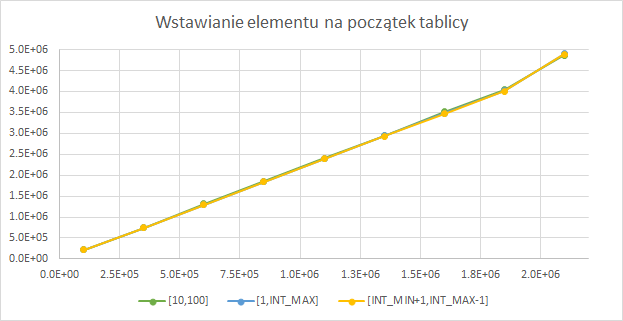
\includegraphics[width=11.3cm]{images/poczatek_wykres.png}
\end{figure}

\newpage
\subsubsection*{Wstawianie elementu w środku}

\begin{figure}[h!]
    \centering
    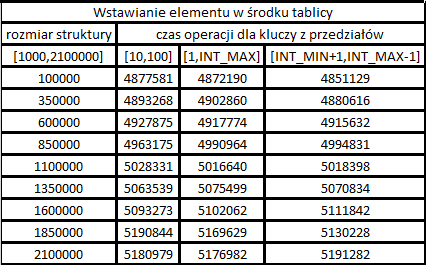
\includegraphics{images/TAB_SRODEK.png}
\end{figure}

\begin{figure}[h!]
    \centering
    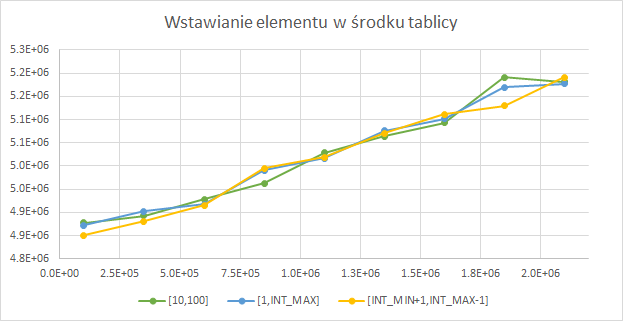
\includegraphics[width=11.3cm]{images/wstawianie_srodek_tab.png}
\end{figure}

\newpage

\subsubsection*{Wstawianie elementu na końcu}

\begin{figure}[h!]
    \centering
    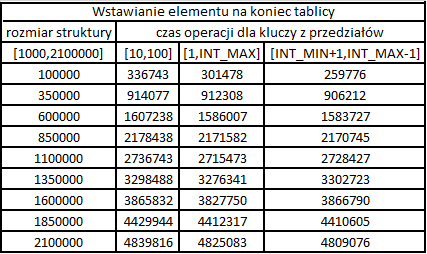
\includegraphics{images/TAB_KONIEC.png}
\end{figure}

\begin{figure}[h!]
    \centering
    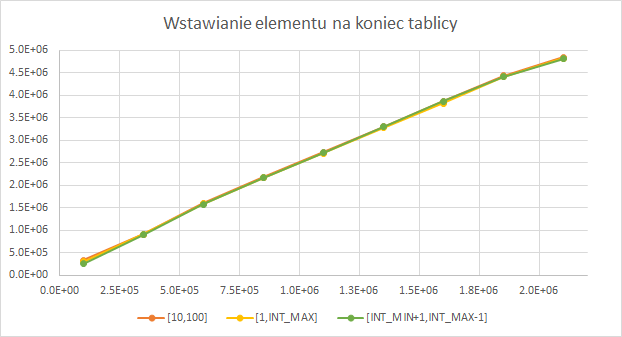
\includegraphics[width=11.3cm]{images/wstawianie_koniec_tab.png}
\end{figure}

\newpage

\subsubsection*{Wyszukiwanie klucza poza przedziałem}

\begin{figure}[h!]
    \centering
    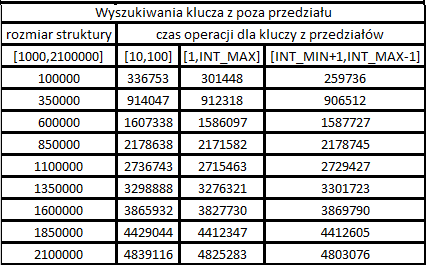
\includegraphics{images/Wyszukiwanie.png}
\end{figure}

\begin{figure}[h!]
    \centering
    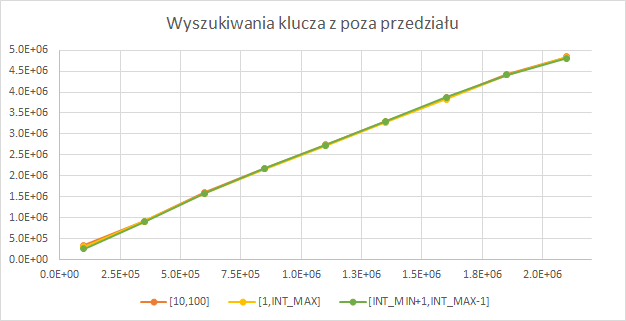
\includegraphics[width=11.3cm]{images/wyszukiwanie_tab.png}
\end{figure}

\newpage

\subsubsection*{Usuwanie elementu z początku}

\begin{figure}[h!]
    \centering
    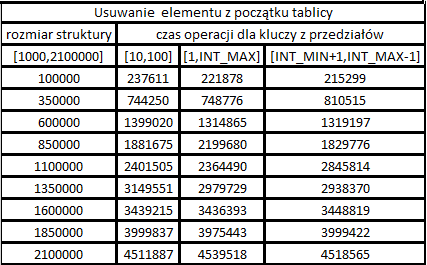
\includegraphics{images/usuwanie_poczatek.png}
\end{figure}

\begin{figure}[h!]
    \centering
    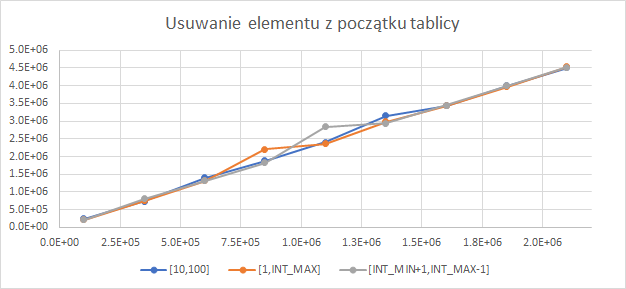
\includegraphics[width=11.3cm]{images/usuwanie_poczatek_tab.png}
\end{figure}

\newpage

\subsubsection*{Usuwanie elementu z środka}

\begin{figure}[h!]
    \centering
    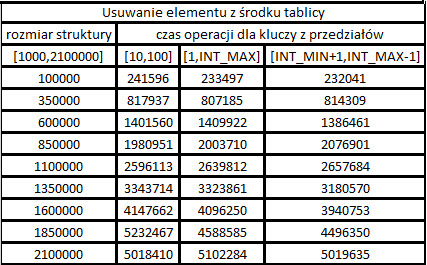
\includegraphics{images/Usuwanie_srodek.png}
\end{figure}

\begin{figure}[h!]
    \centering
    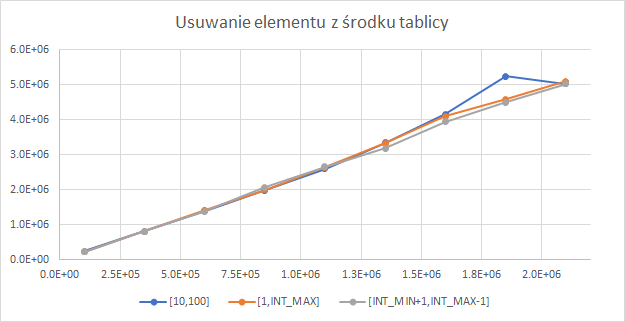
\includegraphics[width=11.3cm]{images/usuwanie_srodek_wykres.png}
\end{figure}

\newpage

\subsubsection*{Usuwanie elementu z końca}

\begin{figure}[h!]
    \centering
    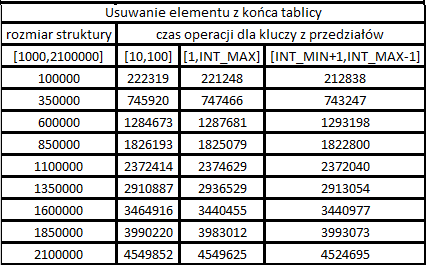
\includegraphics{images/usuwanie_koniec.png}
\end{figure}

\begin{figure}[h!]
    \centering
    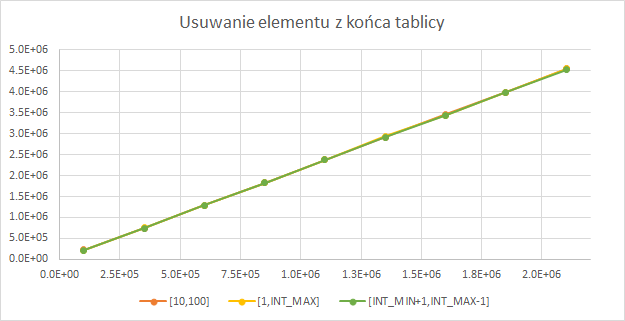
\includegraphics[width=11.3cm]{images/usuwanie_koniec_tab.png}
\end{figure}

\newpage

\subsection{Lista dwukierunkowa}

\subsubsection*{Wstawianie elementu na początek}
\begin{figure}[h!]

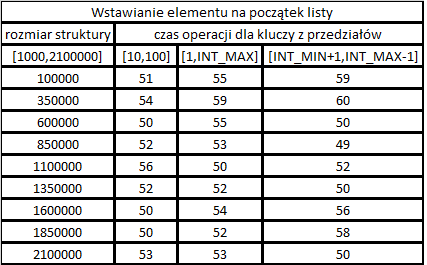
\includegraphics{images/list_dod_pocz.png}

\end{figure}

\begin{figure}[h!]
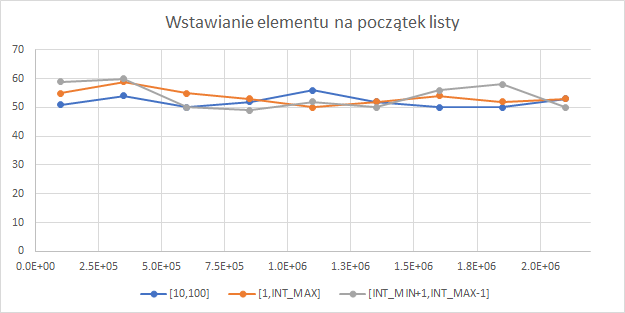
\includegraphics[width=11.3cm]{images/list_dodaj_poczatek_w.png}
\end{figure}

\newpage

\subsubsection*{Wstawienie elementu w środek listy}

\begin{figure}[h!]

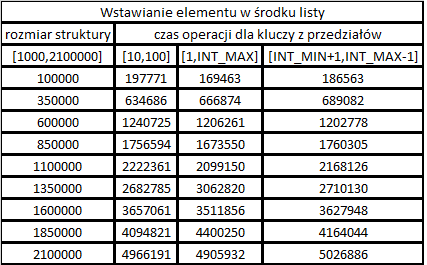
\includegraphics{images/list_wstawianie_srodek_tab.png}

\end{figure}

\begin{figure}[h!]
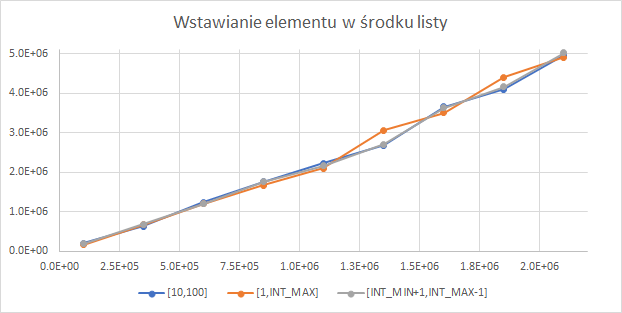
\includegraphics[width=11.3cm]{images/list_wstawianie_srodek_w.png}
\end{figure}

\newpage

\subsubsection*{Wstawienie elementu na koniec listy}

\begin{figure}[h!]

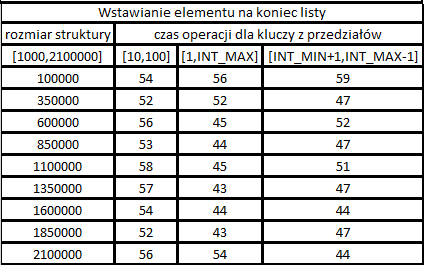
\includegraphics{images/list_dod_koniec.png}

\end{figure}

\begin{figure}[h!]
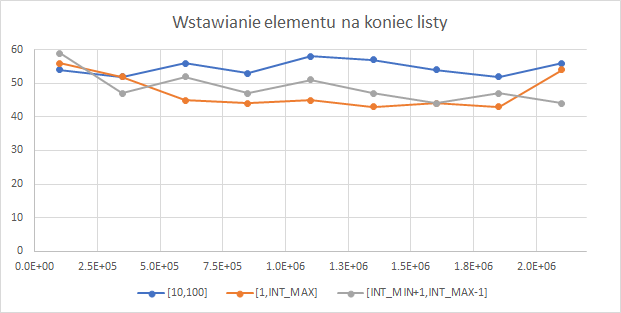
\includegraphics[width=11.3cm]{images/list_dodaj_koniec_w.png}
\end{figure}

\newpage

\subsubsection*{Szukanie elementu w tablicy}

\begin{figure}[h!]

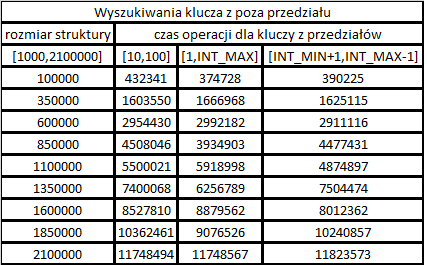
\includegraphics{images/list_Szukanie.png}

\end{figure}

\begin{figure}[h!]
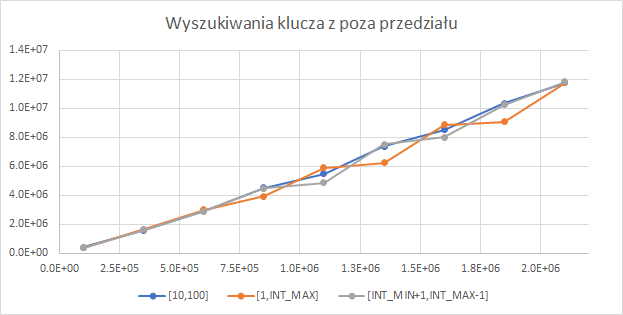
\includegraphics[width=11.3cm]{images/list_wyszukaj_w.png}
\end{figure}

\newpage

\subsubsection*{Usuwanie elementu z początku listy}

\begin{figure}[h!]

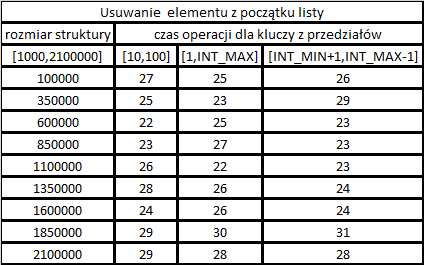
\includegraphics{images/list_usuwanie_pocz.png}

\end{figure}

\begin{figure}[h!]
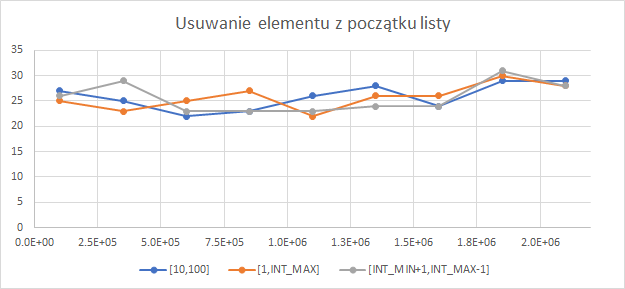
\includegraphics[width=11.3cm]{images/list_usu_pocz_w.png}
\end{figure}

\newpage


\subsubsection*{Usuwanie elementu z środka listy}

\begin{figure}[h!]

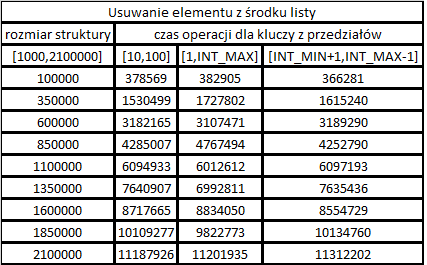
\includegraphics{images/list_usuwanie_srodek_abc.png}

\end{figure}

\begin{figure}[h!]
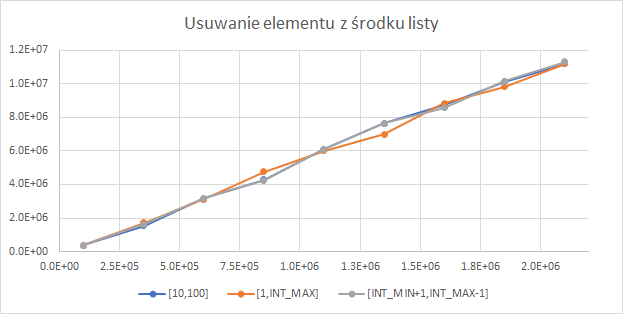
\includegraphics[width=11.3cm]{images/list_usu_srodek_w.png}
\end{figure}

\newpage

\subsubsection*{Usuwanie elementu z końca listy}

\begin{figure}[h!]

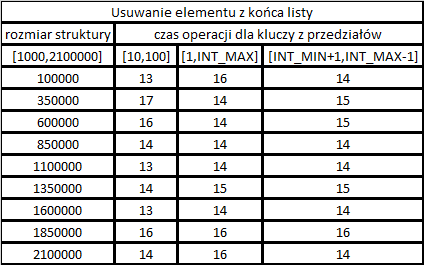
\includegraphics{images/list_usuwanie_koniec.png}

\end{figure}

\begin{figure}[h!]
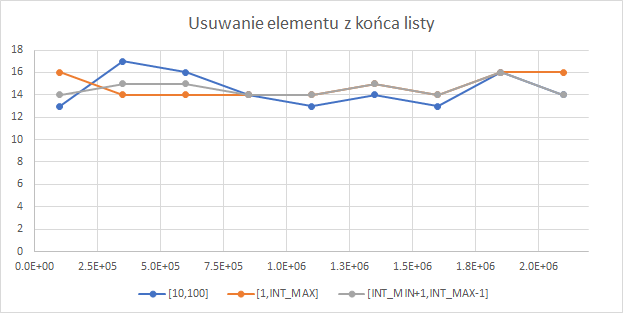
\includegraphics[width=11.3cm]{images/list_usu_koniec_w.png}
\end{figure}

\newpage

\subsection{Kopiec maksymalny}

\subsubsection*{Wstawianie elementu}
\begin{figure}[h!]

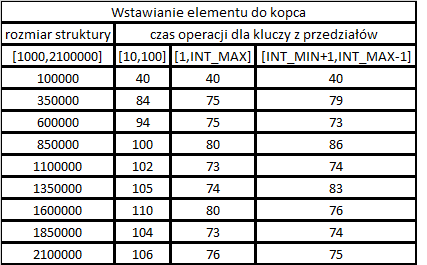
\includegraphics{images/wstawianie_kopiecpng.png}

\end{figure}

\begin{figure}[h!]
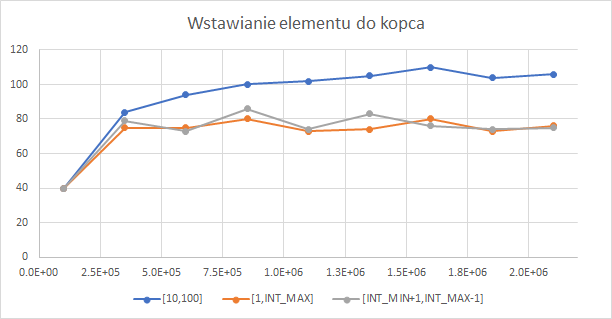
\includegraphics[width=11.3cm]{images/wstawianie_kopiec_w.png}
\end{figure}

\newpage

\subsubsection*{Wyszukiwanie elementu}
\begin{figure}[h!]

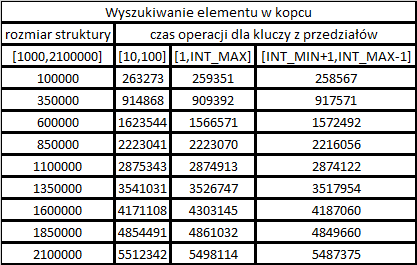
\includegraphics{images/wyszukiwanie_kopiec.png}

\end{figure}

\begin{figure}[h!]
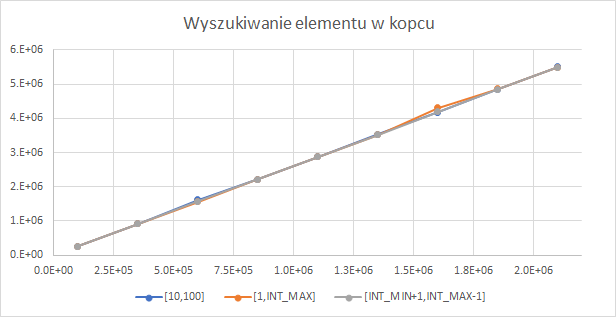
\includegraphics[width=11.3cm]{images/wyszukiwanie_kopiec_w.png}
\end{figure}

\newpage

\subsubsection*{Usuwanie elementu}
\begin{figure}[h!]

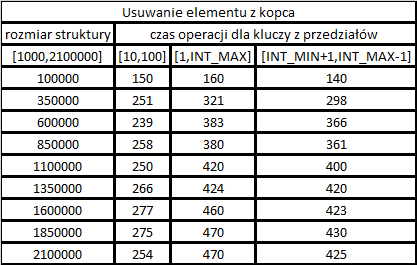
\includegraphics{images/usuwanie_kopiec.png}

\end{figure}

\begin{figure}[h!]
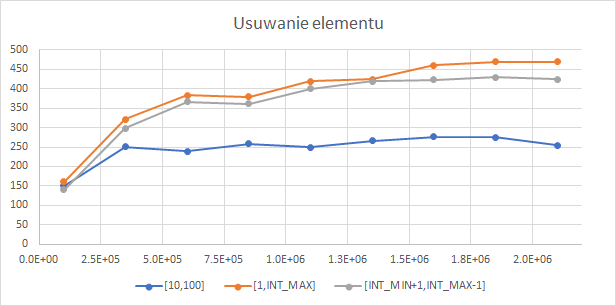
\includegraphics[width=11.3cm]{images/usuwanie_kopiec_w.png}
\end{figure}

\newpage

\subsection{Drzewo BST}

\subsubsection*{Wstawianie elementu}

\begin{figure}[h!]

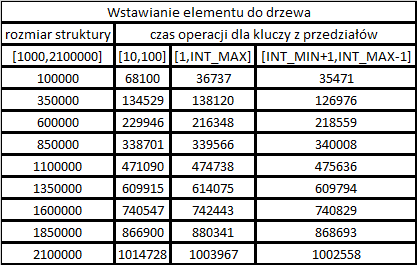
\includegraphics{images/drzewo_wstawianie.png}

\end{figure}

\begin{figure}[h!]
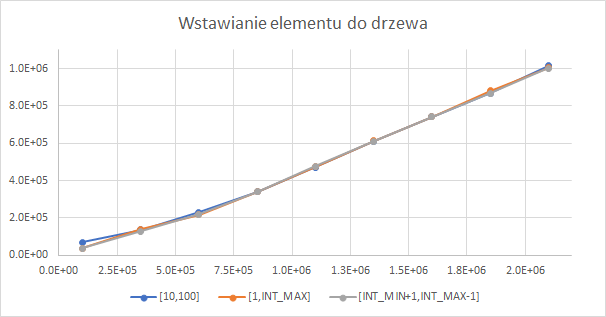
\includegraphics[width=11.3cm]{images/wstawianie_drzewo_w.png}
\end{figure}

\newpage

\subsubsection*{Wyszukiwanie elementu}

\begin{figure}[h!]

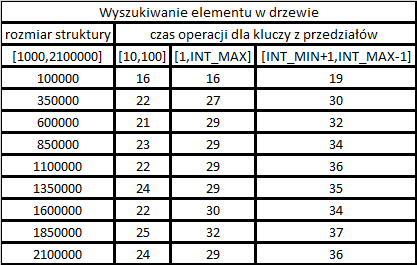
\includegraphics{images/wyszukiwanie_drzewo.png}

\end{figure}

\begin{figure}[h!]
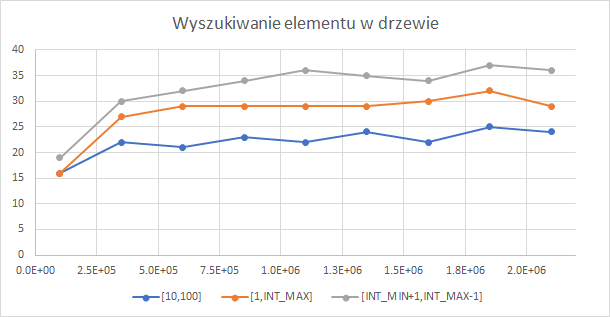
\includegraphics[width=11.3cm]{images/wyszukiwanie_drzewo_w.png}
\end{figure}

\newpage

\subsubsection*{Usuwanie elementu}

\begin{figure}[h!]

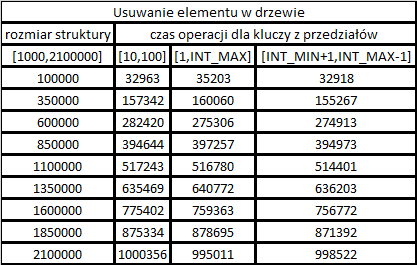
\includegraphics{images/usuwanie_drzewo.png}

\end{figure}

\begin{figure}[h!]
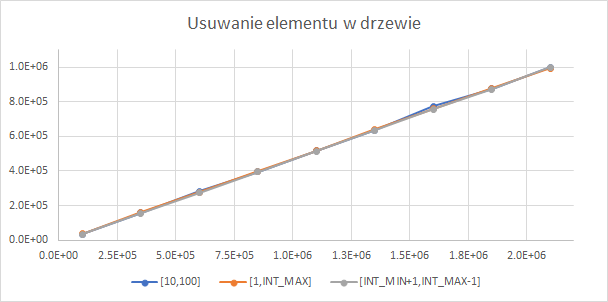
\includegraphics[width=11.3cm]{images/usuwanie_drzewo_w.png}
\end{figure}

\newpage

\section{Wnioski}

Wszystkie badania przebiegły zgodnie z założeniami oraz potwierdziły zgodność teorii z rzeczywistą implementacją danych struktur. Drobne odstępstwa widoczne na wykresach, mieszczą się w zakresie błędów pomiarowych. Wynikają one z nierównej pracy procesora podczas dokonywanych pomiarów. Dla wszystkich struktur nie przybierających postaci drzewiastych, zauważyć można, że przedział przechowywanych kluczy nie ma znaczącego wpływu na szybkość \linebreak wykonywanych operacji. Natomiast operacja dodawania oraz usuwania elementu z kopca zależna jest od kluczy przechowywanych w strukturze, odpowiednio dla dodawania czas dla małych kluczy jest dłuższy natomiast podczas usuwania sytuacja jest odwrotna. Potwierdzeniem teorii jest też wykres przedstawiający rozkład czasów wyszukiwania elementu w drzewie BST względem rozmiaru struktury, ponieważ widać tam silny wpływ przedziału kluczy na czas wykonywania operacji. Wykres przyjął postać logarytmiczną co zgadza się z twierdzeniem mówiącym o logarytmicznym wzroście czasu wyszukiwania względem \linebreak liczby poziomów drzewa.

\end{document}
